% This work is licensed under the Creative Commons
% Attribution-NonCommercial-ShareAlike 4.0 International License. To view a copy
% of this license, visit http://creativecommons.org/licenses/by-nc-sa/4.0/ or
% send a letter to Creative Commons, PO Box 1866, Mountain View, CA 94042, USA.

\chapter{Stoppzeiten und Stoppen von stochastischen Prozessen} %3
%\section{Stoppzeiten}
\begin{defi}[Stoppzeit]\enter
Sei $(\Omega,\A,\P)$ ein Wahrscheinlichkeitsraum mit Filtration $(\F_t)_{t\in I}$. Eine \textbf{Stoppzeit} ist ein zufälliger Zeitpunkt $\tau:\Omega\to I$ mit der Eigenschaft
\begin{align*}
\lbrace\tau\leq t\rbrace:=\lbrace\omega\in\Omega:\tau(\omega)\leq t\rbrace\in\F_t\qquad\forall t\in I
\end{align*}
\ul{Interpretation}: Zu jedem Zeitpunkt $t\in I$ wissen wir, ob $\tau$ bereits eingetreten ist $\lbrace\tau\leq t\rbrace$ oder nicht.
\end{defi}

\begin{beisp}[Typisches Beispiel]\enter
\ul{Ersteintrittszeit} von adaptierten stochastischen Prozessen:
\begin{align*}
\tau:=\min\big\lbrace n\in\N_0:X_n\geq k\big\rbrace
\end{align*}
ist die Ersteintrittszeit in $[k,\infty)$.
\end{beisp}

\setcounter{section}{3}
\begin{proposition}\label{prop3.1}
Seien $\tau,\sigma, \tau_,\tau_2,\ldots$ Stoppzeiten bzgl. einer Filtration $(\F_n)_{n\in\N_0}$. Dann gilt
\begin{enumerate}[label=(\alph*)]
\item $\begin{aligned}
\big\lbrace\omega\in\Omega:\tau(\omega)=n\big\rbrace\in\F_n\qquad\forall n\in\N
\end{aligned}$
\item $\begin{aligned}
\big\lbrace\omega\in\Omega:\tau(\omega)\geq n\big\rbrace\in\F_{n-1}\qquad\forall n\in\N
\end{aligned}$
\item $\begin{aligned}
\vartheta_n:=\indi_{\lbrace n\leq\tau\rbrace}
\end{aligned}$ ist vorhersehbarer stochastischer Prozess
\item $\sigma\wedge\tau,~\sigma\vee\tau$ sind Stoppzeiten
\item $\inf\limits_{n\in\N_0}\tau_n,~\sup\limits_{n\in\N_0}\tau_n$ sind Stoppzeiten
\end{enumerate}
\end{proposition}
\begin{proof}
Siehe Übung (Blatt 2).
\end{proof}

\begin{defi}
	Sei $(X_t)_{t\in I}$ ein $(\F_t)_{t\in I}$-adaptierter stochastischer Prozess und $\tau$ eine Stoppzeit. Wir definieren \textbf{die Zufallsvariable}
\begin{align*}
X_\tau(\omega):=:X_{\tau(\omega)}(\omega)\qquad\forall \omega\in\lbrace\tau<\infty\rbrace
\end{align*} 
und den \textbf{bei $\tau$ gestoppten stochastischen Prozess}
\begin{align*}
X_t^\tau(\omega):=:X_{t\wedge\tau}(\omega):=\left\lbrace\begin{array}{cl}
X_t(\omega), & \falls \omega\in\lbrace t\leq\tau\rbrace\\
X_{\tau(\omega)}(\omega), &\falls\omega\in\lbrace t>\tau\rbrace
\end{array}\right.
\end{align*}
\end{defi}

\begin{bemerkung}
$X^\tau$ ist wieder $(\F_t)_{t\in I}$-adaptiert.
\end{bemerkung}

\begin{theorem}\label{theorem3.2}
Sei $(X_n)_{n\in\N_0}$ ein Martingal und $\tau$ eine Stoppzeit bezgl. $(\F_n)_{n\in\N_0}$.\\
Dann ist der gestoppte Prozess $(X_{n\wedge\tau})_{n\in\N}$ wieder ein Martingal und es gilt
\begin{align}\label{eqTheorem3.2}
\E\big[X_{n\wedge\tau}\big]=\E[X_0]\qquad\forall n\in\N_0
\end{align}
\end{theorem}

\begin{bemerkung}
Das gleiche Resultat gilt für Sub-/Supermartingale mit ``$\geq$'' bzw. ``$\leq$'' in \eqref{eqTheorem3.2}.
\end{bemerkung}

\begin{proof}
In diskreter Zeit können wir das Stoppen als Martingaltransformation mit Integrand
\begin{align*}
\vartheta_n:=\indi_{\lbrace n\leq\tau\rbrace}
\end{align*}
auffassen. Dieser Integrand ist nach Proposition \ref{prop3.1} (c) vorhersehbar. Dann gilt:
\begin{align*}
X_0+(\vartheta\bullet X)_n&=
X_0+\sum\limits_{j=1}^n\indi_{\lbrace j\leq\tau\rbrace}\big(X_j-X_{j-1}\big)\\
&=\left\lbrace\begin{array}{cl}
X_0+\sum\limits_{j=1}^n\big(X_j-X_{j-1}\big)=X_n,&\falls\lbrace\tau\geq n\rbrace\\
X_0+\big(X_1-X_0\big)+\ldots+\big(X_\tau-X_{\tau-1}\big)=X_\tau, &\falls \lbrace\tau<n\rbrace
\end{array}\right.\\
&=X_{\tau\wedge n}
\end{align*}
Die Aussage folgt aus Theorem \ref{theorem2.5}.
\end{proof}

\begin{bemerkung}
Für ein Martingal $X$ gilt also $\E\big[X_{\tau\wedge n}\big]=\E[X_0]$, aber \ul{nicht} unbedingt $\E[X_\tau]=\E[X_0]$.
\end{bemerkung}

\begin{theorem}[Doob's Optional Stopping Theorem]\enter\label{theorem3.3}
Sei $(X_n)_{n\in\N_0}$ ein Martingal und $\tau$ eine endliche Stoppzeit, d. h. $\P[\tau<\infty]=1$. Dann gilt:
\begin{align}\label{eqTheorem3.3}
\E\big[X_\tau\big]=\E\big[X_0\big]
\end{align}
in jedem der folgenden Fälle:
\begin{enumerate}[label=\alph*)]
\item $\begin{aligned}
\tau\text{ ist beschränkt, d. h. }\exists K\in\N_0:\P[\tau\leq K]=1
\end{aligned}$
\item $
\begin{aligned}
X^\tau\text{ ist beschränkt, d. h. }\exists K\geq0:\P\left(\sup\limits_{n\in\N_0}\big| X_{\tau\wedge n}\big|\leq K\right)=1
\end{aligned}$
\item $\begin{aligned}
\E[\tau]<\infty\text{ und }\exists K\geq0:\P\left(\sup\limits_{n\in\N_0}\Big|X_{\tau\wedge n}-X_{\tau\wedge(n-1)}\Big|\leq K\right)=1
\end{aligned}$
\end{enumerate}
\end{theorem}
\begin{proof}
Aus Theorem \ref{theorem3.2} folgt $\E\big[X_{\tau\wedge n}\big]=\E[X_0]$ für alle $n\in\N_0$.\\

\underline{Fall a):}\\
Wähle $n=K$ in \eqref{eqTheorem3.2}:
\begin{align*}
\E[X_0]=\E\big[X_{\tau\wedge n}\big]\stackeq{\tau\leq K}\E[X_\tau]
\end{align*}

\underline{Fall b):} Es gilt
\begin{align*}
\limn X_{n\wedge\tau}=X_\tau\text{ fast sicher und }\big| X_{n\wedge\tau}\big|\leq K\qquad\forall n\in\N
\end{align*}
Mit dominierter Konvergenz
\begin{align*}
\limn\E\big[X_{\tau\wedge n}\big]\stackeq{\text{dom}}\E\left[\limn X_{\tau\wedge n}\right]=\E[X_\tau]
\end{align*}

\underline{Fall c):}
\begin{align*}
\big| X_{n\wedge\tau}-X_0\big|
&\stackeq{\text{Telesk}}
\left|\sum\limits_{j=1}^{n\wedge\tau} X_j-X_{j-1}\right|\\
&\leq\sum\limits_{j=1}^{n\wedge\tau} \underbrace{\big|X_j-X_{j-1}\big|}_{\leq K}\\
&\leq\tau\cdot K
\end{align*}
$\tau\cdot K$ ist integrierbar, da $\E[\tau]<\infty$.
\begin{align*}
\limn\underbrace{\E\big[X_{\tau\wedge n}-X_0\big]}_{=0}\stackeq{\text{domKonv}}\E\big[X_\tau-X_0\big]
\implies
\E\big[X_\tau\big]=\E\big[X_0\big]
\end{align*}
\end{proof}

\begin{beisp}[Einfacher symmetrischer Random Walk]
\begin{align*}
X_n=\sum\limits_{i=1}^n \xi_i\qquad\mit\qquad \P\big(\xi_i=\pm 1\big)=\frac{1}{2}
\end{align*}
Wähle $A,B\in\N$.
\begin{figure}[h!]
	\center
	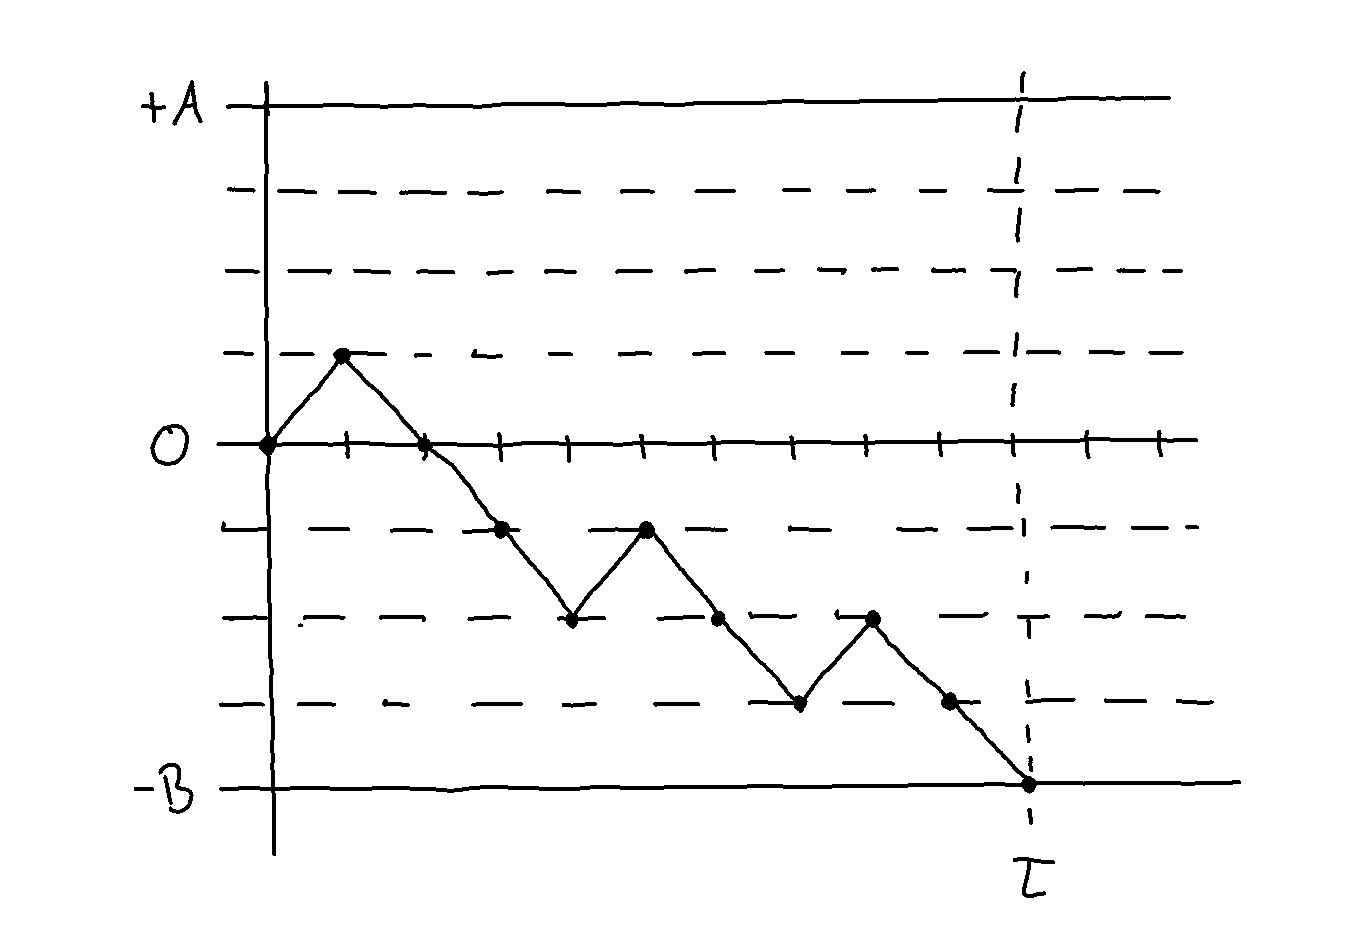
\includegraphics[width=0.75\textwidth]{./pics/Sketch0.png}
	\caption{Ein Random Walk, der eine Eintrittszeit erreicht}
	\label{AbbEintrittszeit}
\end{figure}
\enter
\underline{Fragen:} 
\begin{enumerate}
\item $\P\big( X\text{ erreicht }+A\text{ vor }-B\big)$?
\item $\E\big[\text{ Wartezeit bis }X\text{ Wert }+A\text{ vor }-B\text{ erreicht }\big]$?
\end{enumerate}
Definiere Stoppzeiten 
\begin{align*}
\tau_A&:=\min\big\lbrace n\in\N_0:X_n=+A\big\rbrace\text{ ``Erste Treffzeit von $A$''}\\
\tau_B&:=\min\big\lbrace n\in\N_0:X_n=-B\big\rbrace\text{ ``Erste Treffzeit von $-B$''}\\
\tau&:=\tau_A\wedge\tau_B\text{ ``Erste Treffzeit von $A$ oder $B$``}
\end{align*}
Es gilt $\P[\tau<\infty]=1$  und $\E[\tau]<\infty$ (überprüfen wir beides am Schluss).\\

\underline{Zu Frage 1:}
\begin{align*}
p:=\P\big( X\text{ erreicht }A\text{ vor }-B\big)=\P\big(\tau_A\leq\tau_B\big)
\end{align*}
$X$ ist Martingal, $\big|X_{\tau\wedge n}\big|\leq\max\lbrace A,B\rbrace$. Somit folgt aus Theorem \ref{theorem3.3}:
\begin{align*}
\E\big[X_\tau\big]=\E\big[X_0\big]=0
\end{align*}
Andererseits: 
\begin{align*}
\E\big[X_\tau\big]&=\E\Big[\underbrace{X_{\tau_A}}_{=A}\cdot\indi_{\lbrace\tau_A<\tau_B\rbrace}+\underbrace{X_{\tau_B}}_{=-B}\cdot\indi_{\lbrace\tau_A>\tau_B\rbrace}\Big]\\
&=A\cdot\P\big(\tau_A<\tau_B\big)-B\cdot\P\big(\tau_A>\tau_B\big)\\
&=A\cdot p-B\cdot(1-p)\\
&=p\cdot(A+B)-B\\
&\implies
p=\frac{B}{A+B}
\end{align*}
und somit:
\begin{align*}
\P\big(X\text{ trifft }+A\text{ vor }-B\big)&=\frac{B}{A+B}\\
\P\big(X\text{ trifft }-B\text{ vor }+A\big)&=\frac{A}{A+B}\\
\end{align*}

\underline{Zu Frage 2:}\\
Berechne Kompensator $\langle X\rangle_n$:
\begin{align*}
\E\Big[\underbrace{(X_n-X_{n-1})^2}_{=1}~\Big|~\F_{n-1}\big]=\langle X\rangle_n-\langle X\rangle_{n-1}\\
\implies \langle X\rangle_n=n
\implies M_n=X_n^2-n\text{ ist Martingal}
\end{align*}
Da
\begin{align*}
\big|M_{n\wedge\tau}\big|&\leq
\max\lbrace A^2,B^2\rbrace+\tau
\end{align*}
eine integrierbare (weil $\E[\tau]<\infty$) obere Schranke ist, folgt mit majorierter Konvergenz:
\begin{align*}
\E[M_\tau]&=\limn\E\big[M_{\tau\wedge n}\big]\stackeq{\ref{theorem3.2}}
\E[M_0]=0
\end{align*}
Andererseits:
\begin{align*}
\E[M_\tau]
&=\E\big[X_\tau^2-\tau\big]\\
&=\E\Big[\underbrace{X^2_{\tau_A}}_{=A^2}\cdot\indi_{\lbrace\tau_A<\tau_B\rbrace}+\underbrace{X^2_{\tau_B}}_{=B^2}\cdot\indi_{\lbrace\tau_A>\tau_B\rbrace}\Big] - \E[\tau]\\
&=A^2\cdot\P\big(\tau_A<\tau_B\big)+B^2\cdot\P\big(\tau_B<\tau_A\big)-\E[\tau]\\
&=A^2\cdot\frac{B}{A+B}+B^2\cdot\frac{A}{A+B}-\E[\tau]\\
&=\frac{A^2\cdot B + B^2 \cdot A}{A+B}-\E[\tau]\\
&=A\cdot B-\E[\tau]\\
&\implies
\E[\tau]=A\cdot B
\end{align*}
Also ist $E\big[\text{Wartezeit bis }X\text{ den Wert }+A\text{ oder }-B\text{ erreicht}\big]=A\cdot B$.\\

\underline{Überprüfen von $P(\tau<\infty)=1$:}\\
Definiere Ereignisse
\begin{align*}
\E_k:=\Big\lbrace\omega\in\Omega:X(\omega)\text{ steigt monoton für }k\cdot(A+B)\leq n<(k+1)\cdot(A+B)\Big\rbrace\qquad\forall k\in\N_0
\end{align*}
%TODO Hier Skizze einfügen
Es gilt
\begin{align*}
\omega\in E_k\implies \tau(\omega)\leq(k+1)\cdot(A+B)
\end{align*}
Kontraposition:
\begin{align*}
\tau(\omega)>(k+1)\cdot(A+B)\implies\omega\not\in E_k
\end{align*}
Außerdem: $E_1,E_2,\ldots$ sind unabhängig mit $\P(E_1)=\P(E_2)=\ldots$ und
\begin{align*}
\P(E_1)=2^{-(A+B)}\in(0,1).
\end{align*}
Somit folgt
\begin{align*}
\P\big(\tau>n\cdot(A+B)\big)&=\P\left(\bigcap\limits_{k=0}^n\big\lbrace\tau > k\cdot (A+B)\big\rbrace\right)\\
&\leq\P\left(\bigcap\limits_{k=0}^{n-1} E_k^C\right)\\
&=\Big(1-\P(E_1)\Big)^n\stackrel{n\to\infty}{\longrightarrow}0\\
\P(\tau=\infty)&\leq\underbrace{\P\big(\tau> n\cdot(A+B)\big)}_{\stackrel{n\to\infty}{\longrightarrow}0}\qquad\forall n\in\N_0\\
&\implies
\P(\tau<\infty)=1
\end{align*}

\end{beisp}


